%%%%%%%%%%%%%%%%%%%%%%%%%%%%%%%%%%%%%%%%%%%%%%%%%%%%%%%%%%%%%%%%%%%%%%%%%%%%%%%%%%
\begin{frame}[fragile]\frametitle{}
\begin{center}
{\Large Functions}
\end{center}
\end{frame}

%%%%%%%%%%%%%%%%%%%%%%%%%%%%%%%%%%%%%%%%%%%%%%%%%%%%%%%%%%%
 \begin{frame}[fragile]\frametitle{Functions}
\begin{itemize}
\item Takes many inputs and produces one output
\item $f(x) = x + 2$
\item $f(3)=?$
\item This function is a line, with $y$ is same as $f(x)$
\end{itemize}
\begin{center}
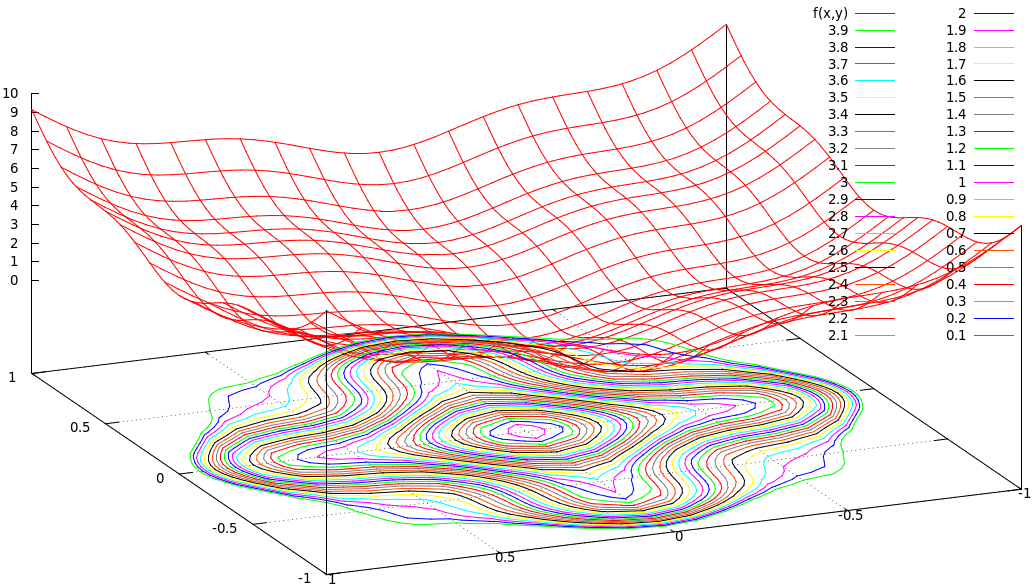
\includegraphics[width=0.5\linewidth,keepaspectratio]{func1}
\end{center}
\end{frame}

%%%%%%%%%%%%%%%%%%%%%%%%%%%%%%%%%%%%%%%%%%%%%%%%%%%%%%%%%%%
 \begin{frame}[fragile]\frametitle{Functions}
\begin{itemize}
\item Another example : $g(x) = 10/x$
\item $g(5)=?$
\item $g(0)=undefined$
\item Set of numbers for which the function is defined is called ``Domain''.
\item For $g$ domain is $\{x \in \mathbb{R} | x \neq 0\}$
\end{itemize}
\begin{center}
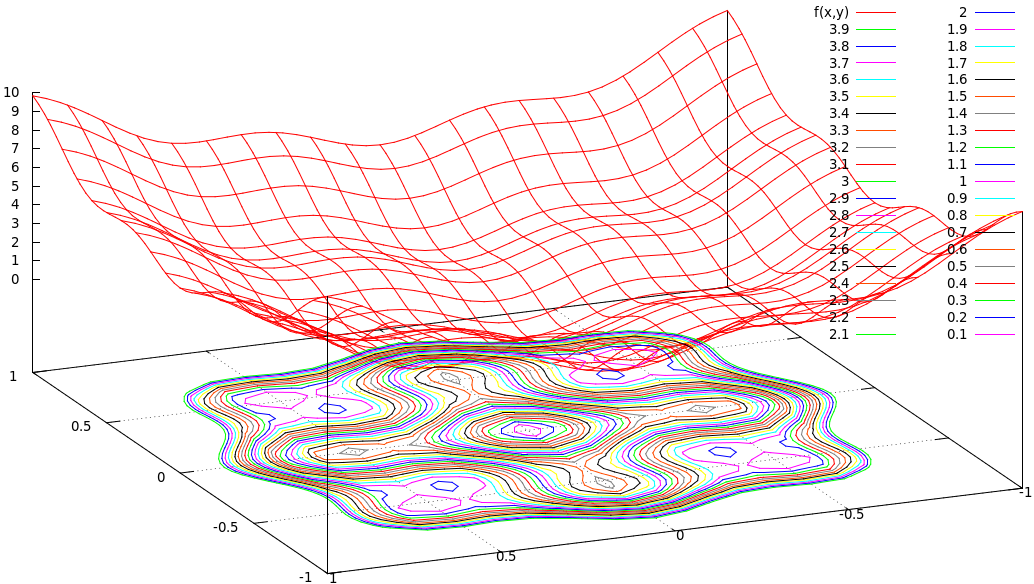
\includegraphics[width=0.5\linewidth,keepaspectratio]{func2}
\end{center}
\end{frame}

%%%%%%%%%%%%%%%%%%%%%%%%%%%%%%%%%%%%%%%%%%%%%%%%%%%%%%%%%%%
 \begin{frame}[fragile]\frametitle{Exercise}
$h(x) = 2 \sqrt{x}, x \geq 0$

Note: Although `domain' is infinite, for plotting, need to restrict it to some range.


\begin{lstlisting}
import numpy as np
from matplotlib import pyplot as plt

def h(x):
    if x >= 0:
        return 2 * np.sqrt(x)

x = range(-100, 101)
y = [h(a) for a in x]

plt.xlabel('x')
plt.ylabel('h(x)')
plt.grid()

plt.plot(x,y, color='purple')
plt.plot(0,h(0.01), color='purple', marker='o')
plt.show()
\end{lstlisting}
\end{frame}

%%%%%%%%%%%%%%%%%%%%%%%%%%%%%%%%%%%%%%%%%%%%%%%%%%%%%%%%%%%
 \begin{frame}[fragile]\frametitle{Plot}
\begin{center}
\includegraphics[width=0.5\linewidth,keepaspectratio]{func3}
\end{center}
\end{frame}


% %%%%%%%%%%%%%%%%%%%%%%%%%%%%%%%%%%%%%%%%%%%%%%%%%%%%%%%%%%%
 % \begin{frame}[fragile]\frametitle{Computable Functions}
% \begin{itemize}
% \item $p(x) = x^2 - 5x + 6$
% \item Computers can easily compute, once $x$ is given, as it involves just multiplications and additions.
% \item Is it easy to compute Trigonometric functions? like $\sin,\cos$.
% \item Right angle triangle definition
% \begin{center}
% \includegraphics[width=0.5\linewidth,keepaspectratio]{trig}
% \end{center}
% \item Is it a complete definition? Can it handle $\theta > 90$?
% \end{itemize}
% \end{frame}

% %%%%%%%%%%%%%%%%%%%%%%%%%%%%%%%%%%%%%%%%%%%%%%%%%%%%%%%%%%%
 % \begin{frame}[fragile]\frametitle{Functions}
% \begin{itemize}
% \item To go beyond $90$ we may use addition formula $\sin(a+b) = \sin a \cos b + \cos a \sin b$
% \item But still, we need formulation thats more encompassing. Thats given by circle.
% \item A real-line is divided into parts of $2\pi$. One of the parts, say $0-2\pi$ is wrapped around a circle with unit radius.
% \item Any real number will have a place on the circumference.
% \item This point's x coordinate gives $\cos number$, y coordinate gives $\sin number$.
% \begin{center}
% \includegraphics[width=0.3\linewidth,keepaspectratio]{circ}
% \end{center}
% \end{itemize}
% \end{frame}


% %%%%%%%%%%%%%%%%%%%%%%%%%%%%%%%%%%%%%%%%%%%%%%%%%%%%%%%%%%%
 % \begin{frame}[fragile]\frametitle{Functions: Series expansion}
% \begin{itemize}
% \item For computers to compute, you need expression in terms of multiplication and additions.
% \item Functions like Trigonometric (Transcendental) are not like that.
% \item Taylor's series (aka Mcluaren) given generic way of expressing functions as series
% \item $f(x=0) = \sum_{n=0}{\infty} \frac{f^n(0)}{n!} x^n$
% \item $\sin x = x - \frac{x^3}{3!} + \frac{x^5}{5!} + \ldots$
% \end{itemize}
% \end{frame}

% %%%%%%%%%%%%%%%%%%%%%%%%%%%%%%%%%%%%%%%%%%%%%%%%%%%%%%%%%%%
% \begin{frame}[fragile]\frametitle{}
% \textbf{Definition}
% A \underline{function of two variables} is a rule which assigns to each pair $(x,y)$ of real numbers in a set $D$ called the \underline{domain} a unique real value denoted by $f(x,y)$.  \\ 
% The set of all values attained by $f$ is the \underline{range} of $f$.
 

% \textbf{Example}
% The area of a rectangle is a function of its length $\ell$ and its width $w$.  So, it can be thought of as a function of two variables $A(\ell,w)=\ell w$.
 

% \textbf{Convention}  
% If an explicit rule is given for a function of two or more variables and the domain is not specified, then the domain is understood to be the set of all possible inputs for which the explicit rule gives a well defined real number.

% \end{frame}



% %%%%%%%%%%%%%%%%%%%%%%%%%%%%%%%%%%%%%%%%%%%%%%%%%%%%%%%%%%%
% \begin{frame}[fragile]\frametitle{}

% \textbf{Example}
% What is the domain of the function $f(x,y)=\ln(x^2-y^2)$?
  

% \textbf{Note}
% If a function arises in an application then the domain maybe determined by the application itself.
  

% \textbf{Example}
% Suppose that $V(r,h)=\pi r^2h$ is the volume of a cylindrical water tank with radius $r$ and height $h$.  What is the domain of $V$.


% \textbf{Example}
% Find the domain and range of the function $f(x,y)= \sqrt{16-x^2-y^2}$.


% \end{frame}

% %%%%%%%%%%%%%%%%%%%%%%%%%%%%%%%%%%%%%%%%%%%%%%%%%%%%%%%%%%%
% \begin{frame}[fragile]\frametitle{}

% \textbf{Definition}
% Suppose that $f(x,y)$ is a function with domain $D$.  The \underline{graph} of $f$ is the set $\{(x,y,f(x,y)) \ |\ (x,y)\in D\}$.
 

% \textbf{Example}
% Draw the graph of the function $h(x,y)= 2x^2 + y^2$.

% \end{frame}

% %%%%%%%%%%%%%%%%%%%%%%%%%%%%%%%%%%%%%%%%%%%%%%%%%%%%%%%%%%%
% \begin{frame}[fragile]\frametitle{}
% \textbf{Definition}
% The \underline{level curves} of a function $f(x,y)$ are the curves in $\mathbb R^3$ with equations $f(x,y)=k$ where $k\in \mathbb R$ is a constant.
 

% \textbf{Note}
% The level curves of $f(x,y)$ are the traces of the graph of $f(x,y)$ in the plane $z=k$.
 

% \textbf{Example}
% Compute the level curves of $f(x,y)=\sqrt{16-x^2-y^2}$.

% \end{frame}

% %%%%%%%%%%%%%%%%%%%%%%%%%%%%%%%%%%%%%%%%%%%%%%%%%%%%%%%%%%%
% \begin{frame}[fragile]\frametitle{}
 
% \textbf{Definition}
 % A \underline{function of $n$ variables} is a rule that assigns to each $n$-tuple $(x_1,\dots, x_n)$ in some subset $D$ or $\mathbb R^n$ a real number $f(x_1,x_2,\dots,x_n)$. \\   
 % The set $D$ is the \underline{domain} of $f$.



% \textbf{Note}
% \begin{enumerate}
 % \item  The graph of a function of $n$ variables naturally lives in $\mathbb R^{n+1}$ which is not easily represented when $n>2$.  
 % \item  When $n=3$, we can gain some insight by considering the level surfaces $f(x,y,z)=k$, where $k\in \mathbb R$ is constant.  
 % \item  When a function of $n$ variables is given by a rule and the domain is not specified we follow the same convention as in the $n=2$ case.  That is, we take the domain to be the set of all values $\vec{x}\in\mathbb R^n$ for which the rule for $f(\vec{x})$ gives a well-defined real number.
% \end{enumerate}

% \end{frame}


% %%%%%%%%%%%%%%%%%%%%%%%%%%%%%%%%%%%%%%%%%%%%%%%%%%%%%%%%%%%
% \begin{frame}[fragile]\frametitle{}
 
% \textbf{Example}
 % Find the domain and range of the function $f(x,y,z)= \ln(16-x^2-y^2-z^2)$.  Plot some of its level surfaces.

% \end{frame}

% %%%%%%%%%%% Supartha Podder %%%%%%%%%%%%%%%%%%%

% \begin{frame}
% \frametitle{Functions}

% \begin{itemize}
% \item $f(x)=y$. 
% %\begin{center}
% % \includegraphics[scale=0.5]{./images/joke1.png}
% %\end{center}

% \end{itemize}

% \end{frame}


% \begin{frame}
% \frametitle{Functions} 

% \begin{block}{Function}
% Let $A$ and $B$ be nonempty sets. $A$ function $f$ from $A$ to $B$ is an assignment of exactly one element of $B$ to each element of $A$.
% \end{block}
% %\pause
% %\begin{center}
% %\includegraphics[scale=0.3]{./images/p1.png}
% %\end{center}
% \end{frame}



% \begin{frame}
% \frametitle{Functions} 

% \begin{block}{Function}
% Let $A$ and $B$ be nonempty sets. $A$ function $f$ from $A$ to $B$ is an assignment of exactly one element of $B$ to each element of $A$.
% \end{block}

% %\begin{center}
% %\includegraphics[scale=0.4]{./images/p2.png}
% %\end{center}
% \pause
% \begin{block}{}
% \begin{itemize}
% \item We write $f(a)=b$ if $b$ is the unique element of $B$ assigned by the function $f$ to the element a of $A$. \pause
% \item If $f$ is a function from $A$ to $B$, we write $f:A\rightarrow B$.
% \end{itemize}
% \end{block}



% \end{frame}



% \begin{frame}
% \frametitle{Function Definitions}
% %\begin{center}
% %\includegraphics[scale=0.4]{./images/p2.png}
% %\end{center}

% \begin{itemize}
% \item If $f$ is a function from $A$ to $B$, we say that $A$ is the domain of $f$ and $B$ is the codomain of $f$. \pause
% \item If $f(a)=b$, we say that $b$ is the image of $a$ and $a$ is a preimage of $b$.  \pause
% \item The range, or image, of $f$ is the set of all images of elements of $A$. \pause
% \item Also, if $f$ is a function from $A$ to $B$, we say that $f$ maps $A$ to $B$.
% \end{itemize}

% \end{frame}




% \begin{frame}
% \frametitle{Function Definitions}


% \begin{block}{Question:}
% What  are  the  domain,  codomain,  and  range  of  the  function  that  assigns  grades  to  students described below?
% %\begin{center}
% %\includegraphics[scale=0.3]{./images/p1.png}
% %\end{center}
% \end{block}\pause



% \begin{itemize}
% \item Let $G$ be the function that assigns a grade to a students. Note that $G($Adams$)=A$, for instance. \pause
% \item The domain of $G$ is the set $\{$Adams, Chou, Goodfriend, Rodriguez, Stevens$\}$, \pause
% \item The codomain is the set $\{A, B, C, D, F\}$.\pause
% \item The range of $G$ is the set $\{A, B, C, F\}$.
% \end{itemize}

% \end{frame}




% \begin{frame}
% \frametitle{Functions}
% %\begin{center}
% %\includegraphics[scale=0.4]{./images/p2.png}
% %\end{center}
% \begin{block}{}
% Let $f$ be the function that assigns the last two bits of a bit string of length 2 or greater to that string. For example, $f(11010)=10$. What are domain, codomain and range?
% \end{block} \pause

% \begin{itemize}
% \item The domain of $f$ is the set of all bit strings of length 2 or greater.\pause
% \item  And both the codomain and range are the set $\{00,01,10,11\}$.
% \end{itemize}

% \end{frame}



% \begin{frame}
% \frametitle{Functions}
% %\begin{center}
% %\includegraphics[scale=0.4]{./images/p3.png}
% %\end{center}
% \begin{block}{}
% Let $f$ be a function from $A$ to $B$ and let $S$ be a subset of $A$. The image of $S$ under the function $f$ is the subset of $B$ that consists of the images of the elements of $S$. We denote the image of $S$ by $f(S)$, so
% \[f(S) = \{ t\textit{ } |\textit{ } \exists s \in S (f(s)=t)\}.\]
% \end{block}
% \end{frame}




% \begin{frame}
% \frametitle{Functions}

% \begin{block}{}
% Let $f_1$ and $f_2$ be functions from $A$ to $\mathbb{R}$. Then $f_1+f_2$ and $f_1\cdot f_2$ are also functions from $A$ to $R$ defined for all $x\in A$ by
% \[(f_1+f_2)(x)=f_1(x)+f_2(x)\]
% \[(f_1\cdot f_2)(x)=f_1(x)\cdot f_2(x).\]

% \end{block} \pause

% \begin{block}{}
% Let $f_1$ and $f_2$ be functions from $\mathbb{R}$ to $\mathbb{R}$ such that $f_1(x)=x^2$ and $f_2(x)=x-x^2$. Then what are $f_1+f_2$ and $f_1\cdot f_2$? \pause

% \[ (f_1+f_2)(x)=f_1(x)+f_2(x)=x^2+(x-x^2)=x\]\pause
% \[ (f_1\cdot f_2)(x)=x^2(x-x^2)=x^3-x^4\]

% \end{block} 
% \end{frame}



 % %----------------------------------------------------------------------------------------
% %	COVER STARTS HERE
% %----------------------------------------------------------------------------------------
% \setbeamertemplate{footline}{}
% \begin{frame}[noframenumbering]
 % \frametitle{}
 % \begin{center}
% \vspace{1cm}
% \Huge{One-to-One Functions}

% \end{center}
% \end{frame}
 % \setbeamertemplate
 % {footline}{\quad\hfill\insertframenumber/\inserttotalframenumber\strut\quad} 
% %----------------------------------------------------------------------------------------
% %	COVER ENDS HERE
% %----------------------------------------------------------------------------------------

 


% \begin{frame}
% \frametitle{One-to-One and Onto Functions}

% %\begin{center}
% %\includegraphics[scale=0.4]{./images/p4.png}
% %\end{center} \pause

% \begin{itemize}
% \item $\forall a \forall b \textit{ } (a \neq b \rightarrow f(a) \neq f(b))$ \pause
% \item $\forall a \forall b \textit{ } (f(a)= f(b) \rightarrow  a = b )$ \pause
% \end{itemize}

% \begin{block}{}
% A function $f:A \rightarrow B$ is said to be one-to-one, or an injunction, if and only if $f(a)=f(b)$ implies that $a=b$ for all $a, b\in A$. A function is said to be injective if it is one-to-one. \pause
% \[\forall a\in A, \forall b\in A \textit{ } (f(a)=f(b) \rightarrow a=b)\]
% \end{block}
% \end{frame}


% \begin{frame}
% \frametitle{Examples of One-to-One and Onto Functions}

% \begin{block}{Question}
% Determine whether $f: \mathbb{Z} \rightarrow \mathbb{Z}$ be defined by $f(x)=x^2$ is one-to-one.
% \end{block} \pause

% \begin{block}{}
% $f$ is not one-to-one because, for instance, $f(1)=f(-1)=1$, but $1\neq -1$. \\
% Note that changing domain to $\mathbb{Z}^+$ makes the function one-to-one.
% \end{block} \pause

% \begin{block}{Question}
% Determine whether $g: \mathbb{R} \rightarrow \mathbb{R}$ such that $g(x)=x+1$ is one-to-one.
% \end{block} \pause

% \begin{block}{}
% The function $g$ is one-to-one. We show this by proving that, 
% \[\forall a \forall b (f(a)= f(b) \rightarrow  a = b )\] \pause

% For any $x, y$ in the domain let $x+1 = y+1$. Then $x= y$. 

% \end{block}
% \end{frame}


% % %----------------------------------------------------------------------------------------
% %%	COVER STARTS HERE
% %%----------------------------------------------------------------------------------------
% %\setbeamertemplate{footline}{}
% %\begin{frame}[noframenumbering]
% % \frametitle{}
% % \begin{center}
% %\vspace{1cm}
% % \includegraphics[scale=0.4]{./images/rec1.png}
% %
% %\end{center}
% %\end{frame}
% % \setbeamertemplate
% % {footline}{\quad\hfill\insertframenumber/\inserttotalframenumber\strut\quad} 
% %%----------------------------------------------------------------------------------------
% %%	COVER ENDS HERE
% %%----------------------------------------------------------------------------------------
% %
% % 

% \begin{frame}
% \frametitle{Proving Injectivitiy or One-to-One}
% \begin{block}{}
% To prove that a function $f:A \rightarrow B$ is injective, it is best to use the definition of injectivity in the second form i.e.,
% \[\forall a \forall b (f(a)= f(b) \rightarrow  a = b )\] \pause
% The first form is sometime difficult to prove as it involves the negated statements.
% \end{block}
% \pause
% \begin{block}{Proof Structure}
% Let $x, y \in A$ be given.\\
% Assume $f(x) =f(y)$\\
% $\cdots$  [Logical deductions] $\cdots$.\\
% Therefore $x=y$.\\
% Hence $f$ is injective.


% \end{block}


% \end{frame}




% \begin{frame}
% \frametitle{Example of Injectivitiy or One-to-One}
% \begin{block}{Question}
% Let $f:\mathbb{Z} \rightarrow \mathbb{Z}$ be defined by $f(x) = 3x+ 7$. Show that $f$ is one-to-one.
% \end{block} \pause

% \begin{block}{}
% Proof: We need to show that for every integers $x$ and~$y, f(x) =f(y) \rightarrow x=y$.\\ \pause
% So, let $x$ and $y$ be integers and suppose that $f(x) =f(y)$. We need to show that $x=y$.\\ \pause

% By assumption we know that $f(x) =f(y)$.\\
% So, substituting in our formula for $f$, $3x+ 7 = 3y+ 7$. \\
% So $3x= 3y$ and therefore $x=y$.

% \end{block}

% \end{frame}




 % %----------------------------------------------------------------------------------------
% %	COVER STARTS HERE
% %----------------------------------------------------------------------------------------
% \setbeamertemplate{footline}{}
% \begin{frame}[noframenumbering]
 % \frametitle{}
 % \begin{center}
% \vspace{1cm}
% \Huge{Onto Functions}

% \end{center}
% \end{frame}
 % \setbeamertemplate
 % {footline}{\quad\hfill\insertframenumber/\inserttotalframenumber\strut\quad} 
% %----------------------------------------------------------------------------------------
% %	COVER ENDS HERE
% %----------------------------------------------------------------------------------------

 

% \begin{frame}
% \frametitle{Onto Functions}
% \begin{block}{Onto}
% A function $f$ from $A$ to $B$ is called onto, or a surjection, if and only if for every element $b\in B$ there is an element $a\in A$ with $f(a)=b$. A function $f$ is called surjective if it is onto. 
% \[\forall y\in B \textit{ } \exists x\in A \textit{ } (f(x)=y)\]
% \end{block}
% %\begin{center}
% %\includegraphics[scale=0.4]{./images/p2.png}
% %\end{center}
% \end{frame}









% \begin{frame}
% \frametitle{Examples of Onto}

% \begin{block}{Question}
% Is the function $f: \mathbb{Z} \rightarrow \mathbb{Z}$ defined by $f(x) =x^2$ onto?
% \end{block} \pause

% \begin{block}{}
% It is not, because there is no interger $x$ with $x^2 =-1$.
% \end{block} \pause

% \begin{block}{Question}
% Is the function $f: A \rightarrow B$, where $A,B$ are $\mathbb{Z}$ defined by $f(x)=x+1$ onto?
% \end{block} \pause

% \begin{block}{}
% This  function  is  onto,  because  for  every  integer $y$ there  is  an  integer $x$ such  that $f(x)=y$.\\
% \pause
% Take any $y \in B$. \\
% Then by definiton, $f(x)=y$ if and only if $x+1=y$.\\
% Hence, $x=y-1$. Since $y\in \mathbb{Z}$, $x \in \mathbb{Z}$.

% \end{block}
% \end{frame}



% % %----------------------------------------------------------------------------------------
% %%	COVER STARTS HERE
% %%----------------------------------------------------------------------------------------
% %\setbeamertemplate{footline}{}
% %\begin{frame}[noframenumbering]
% % \frametitle{}
% % \begin{center}
% %\vspace{1cm}
% % \includegraphics[scale=0.4]{./images/rec1.png}
% %
% %\end{center}
% %\end{frame}
% % \setbeamertemplate
% % {footline}{\quad\hfill\insertframenumber/\inserttotalframenumber\strut\quad} 
% %%----------------------------------------------------------------------------------------
% %%	COVER ENDS HERE
% %%----------------------------------------------------------------------------------------



% \begin{frame}
% \frametitle{Proving Surjectivity or Onto}
% \begin{block}{}
% The definition of surjectivity of function $f: A \rightarrow B$ is 
% \[\forall y\in B \textit{ } \exists x\in A \textit{ } (f(x)=y)\]
% \end{block}
% \pause
% \begin{block}{Proof Structure}
% Let $b\in$ B be given\\
% $\cdots$  [Find an $a$ that maps into the given element $b$.]  ...\\
% $\cdots$ [Show that $f(a) =b$.]  $\cdots$ \\
% Hence $f$ is surjective.
% \end{block}


% \end{frame}






% \begin{frame}
% \frametitle{Example of Onto}
% \begin{block}{Question}
% Let $g: \mathbb{Z} \rightarrow \mathbb{Z}$ be defined by $g(x) = x-8$. Is $g$ onto?
% \end{block} \pause

% \begin{block}{}
% We need to show that for every integer $y$, there is an integer $x$ such that $g(x) =y$.\\ \pause
% So, let $y$ be some arbitrary integer.\\  \pause
% Choose $x$ to be $(y+ 8)$. $x$ is an integer, since it’s the sum of two integers.\\ \pause
% But then $g(x) = (y+ 8)-8 =y$, so we’ve found the required pre-image for~$y$.
% \end{block}

% \end{frame}



% \begin{frame}
% \frametitle{Example of Onto}
% \begin{block}{Question}
% Let $f: \mathbb{Z} \rightarrow \mathbb{Z}$ be defined by $f(x) = 3x+7$. Is $f$ onto?
% \end{block} \pause

% \begin{block}{}
% No.\\
% We need to show that for every integer $y$, there is an integer $x$ such that $f(x) =y$.\\ \pause

% So, let $y$ be some arbitrary integer.\\
% Choose $x$ to be $\frac{(y-7)}{3}$.\\ \pause

% If $f$ was a function from the reals to the reals, we'd be ok at this point, because $x$ would be a good preimage for $y$.\\ \pause

% But since  $f: \mathbb{Z} \rightarrow \mathbb{Z}$ for many $y\in \mathbb{Z}$, $\frac{(y-7)}{3}$ is not an integer.\\

% For example: $y= ?$

% \end{block}

% \end{frame}





% \begin{frame}
% \frametitle{Bijective}

% \begin{block}{Bijection}
% The function $f$ is a one-to-one correspondence, or a bijection, if it is both one-to-one and onto. We also say that such a function is bijective.
% \end{block}

% \end{frame}






% %\begin{frame}
% %\frametitle{Example}
% %
% %\only<1>
% %{
% %\includegraphics[scale=0.53]{./images/p14.png}
% %}
% %\only<2>
% %{
% %\includegraphics[scale=0.53]{./images/p13.png}
% %}
% %\only<3>
% %{
% %\includegraphics[scale=0.53]{./images/p12.png}
% %}
% %\only<4>
% %{
% %\includegraphics[scale=0.53]{./images/p11.png}
% %}
% %\only<5>
% %{
% %\includegraphics[scale=0.53]{./images/p10.png}
% %}
% %\only<6>
% %{
% %\includegraphics[scale=0.53]{./images/p9.png}
% %}
% %\only<7>
% %{
% %\includegraphics[scale=0.53]{./images/p8.png}
% %}
% %\only<8>
% %{
% %\includegraphics[scale=0.53]{./images/p7.png}
% %}
% %\only<9>
% %{
% %\includegraphics[scale=0.53]{./images/p6.png}
% %}
% %\only<10>
% %{
% %\includegraphics[scale=0.53]{./images/p5.png}
% %}
% %\end{frame}



% \begin{frame}
% \frametitle{Inverse Functions}

% \begin{block}{}
% Let $f$ be a one-to-one correspondence from the set $A$ to the set $B$. The inverse function of $f$, $f^{-1}$ is the function that assigns to an element $b$ belonging to $B$ the unique element $a$ in $A$ such that $f(a)=b$. The inverse function of $f$ is denoted by $f^{-1}$. Hence, $f^{-1}(b)=a$ when$f(a)=b$..


% \end{block}
% %\begin{center}
% %\includegraphics[scale=0.5]{./images/p15.png}
% %\end{center}

% Bijectivity = Injectivity + Surjectivity.

% \end{frame}


% \begin{frame}
% \frametitle{Function Composition}

% \begin{block}{Function Composition}
% Let $g$ be a function from the set $A$ to the set $B$ and let $f$ be a function from the set $B$ to the set $C$. The composition of the functions $f$ and $g$, denoted for all $a\in A$ by $f\circ g$, is defined by
% \[(f \circ g) (a) = f(g(a))\]
% \end{block}

% %\begin{center}
% %\includegraphics[scale=0.45]{./images/p16.png}
% %\end{center}
% \end{frame}


% \begin{frame}
% \frametitle{Function Composition Example}

% \begin{block}{Question}
% Let $f$ and $g$ be  the  functions  from  the  set  of  integers  to  the  set  of  integers  defined  by $f(x)=2x+3$ and $g(x)=3x+2$. What is the composition of $f$ and $g$? 
% \end{block} \pause

% \begin{block}{}
% \[ (f\circ g)(x) = f(g(x)) = f(3x+2) = 2(3x+2) = 6x+7.\]
% \end{block}
% \end{frame}



% \begin{frame}
% \frametitle{One-to-One and Onto Functions}

% %\begin{center}
% %\includegraphics[scale=0.4]{./images/p4.png}
% %\end{center} 


% \begin{block}{}
% A function $f:A \rightarrow B$ is said to be one-to-one, or an injunction, if and only if $f(a)=f(b)$ implies that $a=b$ for all $a, b\in A$. A function is said to be injective if it is one-to-one.
% \[\forall a\in A, \forall b\in A \textit{ } (f(a)=f(b) \rightarrow a=b)\]
% \end{block}
% \end{frame}

 

% \begin{frame}
% \frametitle{Onto Functions}
% \begin{block}{Onto}
% A function $f$ from $A$ to $B$ is called onto, or a surjection, if and only if for every element $b\in B$ there is an element $a\in A$ with $f(a)=b$. A function $f$ is called surjective if it is onto. 
% \[\forall y\in B \textit{ } \exists x\in A \textit{ } (f(x)=y)\]
% \end{block}
% %\begin{center}
% %\includegraphics[scale=0.4]{./images/p2.png}
% %\end{center}
% \end{frame}






% %\begin{frame}
% %\frametitle{Example}
% %
% %\includegraphics[scale=0.53]{./images/p5.png}
% %
% %\end{frame}





% \begin{frame}
% \frametitle{Example of Bijective Function}

% \begin{block}{}
% Let $f: (\mathbb{R}^+ \times \mathbb{R}^+) \rightarrow (\mathbb{R}^+ \times \mathbb{R}^+)$ be the function defined by $f(r,s) = (2r, rs)$. Proof that $f$ is bijective.
% \end{block}


% \begin{block}{Proof of Injectivity}
% \pause

% Let $(a,b), (c,d) \in \mathbb{R}^+ \times \mathbb{R}^+$ be arbitrary elements of $f$'s domain.\\ \pause
% Assume $f(a,b) = f(c,d)$ (Goal is to prove $(a,b)=(c,d)$.)\\ \pause

% Then, $(2a, ab) = (2c,cd)$\\
% $\Rightarrow 2a=2c$ and $ab=cd$.\\ \pause
% For two ordered pairs to be equal, both their 1st and 2nd coordinates must be equal.\\ \pause

% Thus, $a=c$ and $ab-cd=0$.\\
% $\Rightarrow ab-ad=0$ since $a=c$\\
% $\Rightarrow a(b-d)=0$.\\ \pause

% So, $a=0$ or $b=d$. Now $a=0$ is not possible because of the domain. So $b=d$.\\
% Hence $f$ is injective.

% \end{block}

% \end{frame}





% \begin{frame}
% \frametitle{Example of Bijective Function}

% \begin{block}{}
% Let $f: (\mathbb{R}^+ \times \mathbb{R}^+) \rightarrow (\mathbb{R}^+ \times \mathbb{R}^+)$ be the function defined by $f(r,s) = (2r, rs)$. Proof that $f$ is bijective.
% \end{block}


% \begin{block}{Proof of Surjectivity}
% \pause

% Let $(u,v) \in \mathbb{R}^+ \times \mathbb{R}^+ $ be an arbitrary element of $f$'s co-domain. \\
% We want to find at least one element $(r,s) \in \mathbb{R}^+  \times \mathbb{R}^+ $ (in $f$'s domain) such that $f(r,s)=(u,v)$.\\ \pause

% Well, $f(r,s) = (u,v) \Leftrightarrow (2r, rs) =(u,v)$\\ \pause
% $\Leftrightarrow 2r=u$ and $rs=v$.\\ \pause
% $\Leftrightarrow r=\frac{u}{2}$ and $s=\frac{v}{r}$.\\ \pause
% Thus, $s=\frac{v}{(\frac{u}{2})} = \frac{2v}{u}$. \\

% Now we need to make sure that $(r,s) = (\frac{u}{2}, \frac{2v}{u}) \in \mathbb{R}^+ \times \mathbb{R}^+ $.\\ \pause
% Since $u \in \mathbb{R}^+ $, so is $\frac{u}{2}$ and since $u,v \in \mathbb{R}^+ $ so is $\frac{2u}{v}$.\\ \pause
% Thus $f(\frac{u}{2}, \frac{2v}{u}) = (r,s)$ and $f$ is surjective. 



% \end{block}

% \end{frame}





% \begin{frame}
% \frametitle{Inverse Functions}

% \begin{block}{}
% Let $f$ be a one-to-one correspondence from the set $A$ to the set $B$. The inverse function of $f$, $f^{-1}$ is the function that assigns to an element $b$ belonging to $B$ the unique element $a$ in $A$ such that $f(a)=b$. The inverse function of $f$ is denoted by $f^{-1}$. Hence, $f^{-1}(b)=a$ when$f(a)=b$..


% \end{block}
% %\begin{center}
% %\includegraphics[scale=0.5]{./images/p15.png}
% %\end{center}

% Bijectivity = Injectivity + Surjectivity.

% \end{frame}

% \begin{frame}
% \frametitle{Example of Inverse}

% \begin{block}{}
% Is $f: \mathbb{Z}^2 \rightarrow \mathbb{Z}^2$ defined by $f(x,y)=(x-y, -x)$ invertible?
% \end{block}

% \begin{block}{Injective:}

% Let $(p,q), (r,s) \in \mathbb{Z} \times \mathbb{Z}$ be arbitrary elements of $f$'s domain.\\ \pause
% Assume $f(p,q) = f(r,s)$ (Goal is to prove $(p,q)=(r,s)$.)\\ \pause

% Then, $(p-q, -p) = (r-s,-r)$ \pause $\Rightarrow p=r$ and $q=s$ \pause thus, $(p,q)=(r,s)$.
% \end{block}
% \pause 
% \begin{block}{Surjectivity:}
% Let $(u,v) \in \mathbb{Z} \times \mathbb{Z} $ be an arbitrary element of $f$'s co-domain. \\
% We want to find at least one element $(r,s) \in \mathbb{Z}  \times \mathbb{Z} $ (in $f$'s domain) such that $f(r,s)=(u,v)$.\\ \pause
% By definition of $f$, $(u,v) = (r-s, -r)$, thus $v=-r$ and $u=r-s$.\\ \pause
% $\Rightarrow r=-v$ and $s= -(u+v)$. And since $(u,v) \in \mathbb{Z} \times \mathbb{Z}$, $(r,s) \in \mathbb{Z} \times \mathbb{Z}$,\\ \pause
% and $f(r,s)=(u,v)$.



% \end{block}
% \end{frame}




% \begin{frame}
% \frametitle{Example of Inverse}

% \begin{block}{}
% Is $f: \mathbb{Z}^2 \rightarrow \mathbb{Z}^2$ defined by $f(x,y)=(x-y, -x)$ invertible?
% \end{block}

% \begin{block}{Inverse}
% Now that we have proven bijectivity. Let us find $f^{-1}$. \\ \pause

% We know that $f(x,y) = (r,s)$ hence we need to design the inverse, $f^{-1}(r,s)=(x,y)$. \\ \pause
% Accordin to $f$, $f(x,y)=(x-y, -x) =(r,s)$.\\
% thus $x-y =r$ and $-x=s$.\\
% $\Rightarrow x=-s$ and $y= -s -r$.\\ \pause

% Hence, $f^{-1}(r,s) = (-s, -s-r)$. \\ \pause

% $f^{-1}(x-y,-x) = (x, x-x+y)=(x,y)$.


% \end{block}
% \end{frame}




% \begin{frame}
% \frametitle{Function Composition}

% \begin{block}{Function Composition}
% Let $g$ be a function from the set $A$ to the set $B$ and let $f$ be a function from the set $B$ to the set $C$. The composition of the functions $f$ and $g$, denoted for all $a\in A$ by $f\circ g$, is defined by
% \[(f \circ g) (a) = f(g(a))\]
% \end{block}

% %\begin{center}
% %\includegraphics[scale=0.45]{./images/p16.png}
% %\end{center}
% \end{frame}


% \begin{frame}
% \frametitle{Function Composition Example}

% \begin{block}{Question}
% Let $f$ and $g$ be  the  functions  from  the  set  of  integers  to  the  set  of  integers  defined  by $f(x)=2x+3$ and $g(x)=3x+2$. What is the composition of $f$ and $g$? 
% \end{block} \pause

% \begin{block}{}
% \[ (f\circ g)(x) = f(g(x)) = f(3x+2) = 2(3x+2) = 6x+7.\]
% \end{block}
% \end{frame}


% \begin{frame}
% \frametitle{Function Composition Example}

% \begin{block}{}
% Let $f$ and $g$ be functions defined as $f: \mathbb{Q}^2 \rightarrow \mathbb{Q}^2$, $g: \mathbb{Q} \rightarrow \mathbb{Q}^2$ such that $f(q,r)=(q+r, 2q)$ and $g(x)=(3x, 5-x)$.
% \end{block}

% \begin{block}{Does $f\circ g$ exist?}
% \pause Yes, $f\circ g: \mathbb{Q} \rightarrow \mathbb{Q}^2$. \\ 

% $f\circ g(x) = f(g(x))$. \pause $= f(3x, 5-x)$\pause $= (3x+5-x, 2(3x))$ \pause $=(2x+5, 6x)$.\\
% $f\circ g(x) = (2x+5, 6x)$.

% \end{block}\pause

% \begin{block}{Does $g\circ f$ exist?}
% \pause No. Because co-domain of $f$ is $\mathbb{Q}^2$ but the domain of $g$ is $\mathbb{Q}$.
% \end{block}

% \end{frame}

% \begin{frame}
% \frametitle{Composition}

% \begin{block}{}
% Let $A$, $B$ and $C$ be sets, and let $f: A\rightarrow B$ and $g: B\rightarrow C$ be two functions. Prove that if $f$ and $g$ are both surjective, then $g\circ f$ is surjective.
% \end{block}\pause

% \begin{block}{}

% Assume that both $f$ and $g$ are surjective. \\ \pause

% Then, \\
% \begin{enumerate}
% \item For each $b\in B$ there exists an element $a\in A$ such that $f(a)=b$ because $f$ is surjective.  \pause
% \item For each $c\in C$ there exists an element $b\in B$ such that $g(b)=c$ because $g$ is surjective. 
% \end{enumerate} \pause

% Note that $g\circ f: A \rightarrow C$.\\ \pause
% Now, take $c \in C$, then $g\circ f(a) = g(f(a))$\pause $=g(b)$ (by (1))\\ \pause $=c$ (by (2)). \\

% Thus, $g\circ f$ is surjective.

% \end{block}
% \end{frame}





% \begin{frame}
% \frametitle{Composition}

% \begin{block}{}
% Show that if $g \circ f$ is surjective then $g$ is surjective.
% \end{block} \pause
% \begin{block}{}
% Suppose that $g \circ f$ is surjective. \\ \pause
% Let $z \in  C$. \\
% Then since $g \circ f$ is surjective, there exists $x \in A$ such that $(g \circ f )(x) = g(f (x)) = z$.\\ \pause

% Therefore if we let $y = f (x) \in B$, then $g(y) = z$.\\ \pause 

% Thus $g$ is surjective.
% \end{block}

% \end{frame}



% \begin{frame}
% \frametitle{Composition}

% \begin{block}{}
% In each part of the exercise, give examples of sets $A, B, C$ and functions $f : A \rightarrow B$
% and $g : B \rightarrow C$ satisfying the indicated properties.

 
% \begin{itemize}
% \item [(a)] $g$ is not injective but $g \circ f$ is injective.

% \item [(b)] $f$ is not surjective but $g \circ f$ is surjective.
% \end{itemize}
 % \pause
% \end{block}
% \begin{block}{}
% The same example works for both.\\ Let $A = \{1\}, B = \{1, 2\}, C = \{1\}$, and $f : A \rightarrow B$
% by $f (1) = 1$ and $g : B \rightarrow C$ by $g(1) = g(2) = 1$.\\ \pause
 % Then $g \circ f : A \rightarrow C$ is defined by $(g \circ f )(1) = 1$. \\ \pause
% This map is a bijection from $A = \{1\}$ to $C = \{1\}$, so is injective and surjective.\\ \pause
% However, $g$ is not injective, since $g(1) = g(2) = 1$, and $f$ is not surjective, since $2 \notin f (A) = {1}$.
% \end{block}
% \end{frame}



% \begin{frame}
% \frametitle{Composition}


% \begin{block}{}
% Define functions $f$ and $g$ from $\mathbb{Z}$ to $\mathbb{Z}$ such that $f$ is not surjective and yet $g \circ f$ is surjective.
% \end{block}
% \pause

% Let,\\
% %\begin{center}
% %
% %\includegraphics[scale=0.4]{./images/soln5.png}\\
% %\end{center} 
% The map $f$ is not surjective: the image is the set of even integers. However, $g \circ f$ is surjective, since $(g \circ f )(n) = g(f (n)) = g(2n)) = (2n)/2 = n$ so in fact $g \circ f$ is the identity map on $\mathbb{Z}$.

% \end{frame}


% %----------------------------------------------------------------------------------------
%%	COVER STARTS HERE
%%----------------------------------------------------------------------------------------
%\setbeamertemplate{footline}{}
%\begin{frame}[noframenumbering]
% \frametitle{}
% \begin{center}
%\vspace{2cm}
% \huge Thank you for your attention!! 
%
%\end{center}
%\end{frame}
% \setbeamertemplate
% {footline}{\quad\hfill\insertframenumber/\inserttotalframenumber\strut\quad} 
%%----------------------------------------------------------------------------------------
%%	COVER ENDS HERE
%%----------------------------------------------------------------------------------------
%
% 



%----------------------------------------------------------------------------------------
%	COVER STARTS HERE
%----------------------------------------------------------------------------------------
%\setbeamertemplate{footline}{}
%\begin{frame}[noframenumbering]
% \frametitle{}
% \begin{center}
%\Huge 
%\end{center}
%\end{frame}
% \setbeamertemplate
% {footline}{\quad\hfill\insertframenumber/\inserttotalframenumber\strut\quad} 
%----------------------------------------------------------------------------------------
%	COVER ENDS HERE
%----------------------------------------------------------------------------------------














%----------------------------------------------------------------------------------------
%              END OF DOCUMENT
%----------------------------------------------------------------------------------------

% \end{document} 

% %----------------------------------------------------------------------------------------













%
%
%\begin{frame}
%\frametitle{Ven Diagram}
%\pagestyle{empty}
%\def\firstcircle{(0,0) circle (1.5cm)}
%\def\secondcircle{(60:2cm) circle (1.5cm)}
%\def\thirdcircle{(0:2cm) circle (1.5cm)}
%\def\rect{(0,0) rectangle (3cm)}
%
%\begin{tikzpicture}
%    \begin{scope}[shift={(3cm,-5cm)}, fill opacity=1]
%        \fill[white] \firstcircle;
%
%
%\fill[black] (-2.01,-2.01) rectangle (2.02,2.02);
%\fill[white] (-2,-2) rectangle (2,2);
%                \fill[white] \firstcircle;
%        \draw \firstcircle node[below] {$a$ $e$  $i$ $o$ $u$};
%    \end{scope}
%\end{tikzpicture}
%\end{frame}
%
%
%
%
%
%
%
%\begin{frame}
%\frametitle{Ven Diagram}
%\pagestyle{empty}
%
%\begin{tikzpicture}
%    \begin{scope}[shift={(3cm,-5cm)}, fill opacity=1]
%        \fill[red] \firstcircle;
%        \fill[green] \secondcircle;
%        \fill[blue] \thirdcircle;
%
%\fill[gray] (-1.7,-2) rectangle (3.7,3.7);
%
%        \draw \firstcircle node[below] {$A$};
%        \draw \secondcircle node [above] {$B$};
%        \draw \thirdcircle node [below] {$C$};
%    \end{scope}
%\end{tikzpicture}
%\end{frame}
%
%


